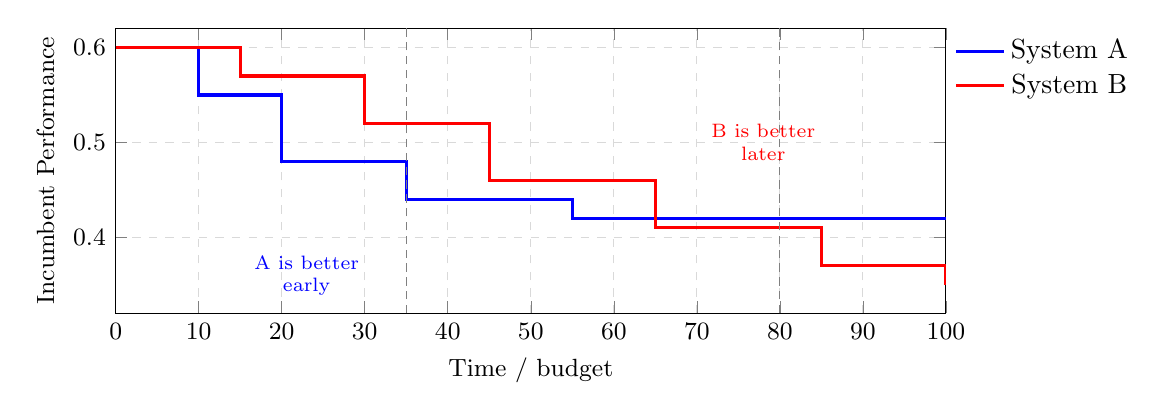
\begin{tikzpicture}
\begin{axis}[
    width=\linewidth,
    height=5.2cm,
    xmin=0, xmax=100,
    ymin=0.32, ymax=0.62,
    xlabel={Time / budget},
    ylabel={Incumbent Performance},
    ymajorgrids=true,
    xmajorgrids=true,
    grid style={dashed,gray!30},
    legend style={
        at={(1,1)},
        anchor=north west,
        draw=none,
        fill=none
    },
    tick label style={font=\small},
    label style={font=\small},
]

% System A: fast decrease, early plateau (worse final loss)
\addplot[
    very thick,
    blue,
    const plot
] coordinates {
    (0,0.60)
    (10,0.55)
    (20,0.48)
    (35,0.44)
    (55,0.42)
    (100,0.42)
};
\addlegendentry{System A}

% System B: slower decrease, better final loss
\addplot[
    very thick,
    red,
    const plot
] coordinates {
    (0,0.60)
    (15,0.57)
    (30,0.52)
    (45,0.46)
    (65,0.41)
    (85,0.37)
    (100,0.35)
};
\addlegendentry{System B}

% Early and late budget markers
\draw[densely dashed,gray] (axis cs:35,0.32) -- (axis cs:35,0.62);
\draw[densely dashed,gray] (axis cs:80,0.32) -- (axis cs:80,0.62);

% Annotations
\node[blue, font=\scriptsize, align=center] at (axis cs:23,0.36)
    {A is better\\early};
\node[red, font=\scriptsize, align=center] at (axis cs:78,0.50)
    {B is better\\later};

\end{axis}
\end{tikzpicture}